\subsection{Chapter 3}

\textbf{Density of States (1D)}

We start with the 1-D wave equation:
$$\frac{\partial^2 u}{\partial x^2} - \frac{\rho}{Y} \frac{\partial u}{\partial t} = 0$$

Which delivers a solution in the way of:\\
(The time depence is not needed for calculatiing the density of states)
\begin{equation}
    u = Ae^{ikx}
    \label{eq:sol_1d_wave}
\end{equation}

By using the boundary conditions:
$$u(x=0) = u(x=L)$$

We get:
$$e^{ikL} = 1$$

Due to Eulers-Equation we get for $k$
$$k = n \frac{2\pi}{L}$$

If you choose integer values for $n$ and plot them along a $k$-axis, they form
a one-dimensional mesh with a constants spacing $(2\pi/L)$ between the poins.

\begin{figure}[H]
	\centering
	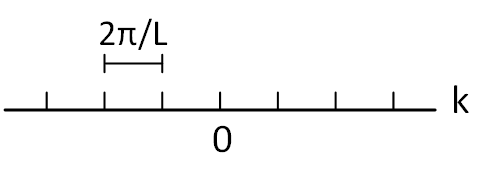
\includegraphics[width=0.4\linewidth]{Graphics/Chapter3/allowed_values_k_1D}
	\caption{Allowed values of $k$}
	\label{}
\end{figure}

As we can see if $L$ becomes large we get quasi-continous points for $k$. So the 
number of modes (points) in an interval $dk$ in $k$-space equals:

$$\dfrac{L}{2\pi} dk$$

Using the dispersion relation we can find the number of modes in a frequency
range $d\omega$, which lies within $(\omega, \omega + d\omega)$.
This number is given as $(g\omega)d\omega$, with
$g(w)$ defined as the density of states.

$$g(\omega) d\omega =\dfrac{L}{2\pi} dk$$

By solving for $g(\omega)$ and multipling with a factor of two.
(Due to the fact that we have to include the modes lying the negative k-region)\\
We get:

\begin{equation}
    g(\omega) = \frac{L}{\pi} \frac{1}{\frac{d\omega}{d k}}
\end{equation}

By assuming that the dispersion in linear $(\omega = v_sk)$ 
the density of states is

\begin{equation}
    g(\omega) = \frac{L}{\pi} \frac{1}{v_s}
\end{equation}

which is independet of $\omega$

\textbf{Density of States (3D)}

Starting with the solution for the wave equation as same as in the 1-D case
(\autoref{eq:sol_1d_wave}) we get:

\begin{equation}
    u = Ae^{i(k_x x + k_y y + k_z z)}
\end{equation}

By applying the same boundary conditions as in the 1-D case we get:

$$u = e^{i(k_x x + k_y y + k_z z)} = 1$$

$$(k_x, \, k_y,\, k_z) = (n \frac{2\pi}{L}, \, m \frac{2\pi}{L}, \, l \frac{2\pi}{L})$$

Each point in this $k$-space has a volume of $(2\pi/L)^3$. The number of
modes that lie within a spherical shell with thikness $dk$ with a radius k 
and a volume $4/3\pi k^3$, is given by:

$$\frac{d}{dk}{(\frac{L}{2\pi})}^3\frac{4}{3}\pi k^3 = {(\frac{L}{2\pi})}^3 4\pi k^2 dk$$

And so with $L^3 = V$:

$$ g(\omega) d \omega =  \frac{V}{2\pi^2} k^2 dk \quad \Rightarrow \quad g(\omega) = \frac{V}{2\pi^2} k^2 \frac{dk}{d \omega} $$

By applying the linear dispersion relation, we get:

\begin{equation}
    g(\omega) = \frac{V}{2\pi^2} \frac{\omega^2}{v_s^3}
    \label{eq:g_ome_3d_1}
\end{equation}

As there are three different modes associated with the same value for $q$.
(one longitudinal and 2 transversal modes). \autoref{eq:g_ome_3d_1} has to be
multiplied by a factor of three to get the correct result.

\begin{equation}
    g(\omega) = \frac{3V}{2\pi^2} \frac{\omega^2}{v_s^3}
\end{equation}


\textbf{Debye Frequency}

In the Debye model the vibration frequency of the lattice covers
a wide rang of values.

The total energy of the lattice is calculated by:

\begin{equation}
    E = \int \overline{\epsilon}(\omega) g(\omega) \, d\omega
    \label{eq:debye_energy}
\end{equation}

$g(\omega) \quad ... \quad \textrm{density of states}$\\
$\overline{\epsilon}(\omega) \quad ... \quad \textrm{energy of each mode}$

For various reasons a cutoff frequency is needed for example to not get
infinit energys in \autoref{eq:debye_energy}.

The upper cutoff frequency was defined, by requiring that the total number of 
modes included must be equal to the number of degrees of freedom for the entire
solid.

\begin{equation}
    \int_0^{\omega_D} g(\omega) \, d\omega = 3N_A
    \label{eq:debye_frequency_int}
\end{equation}

With inserting the \autoref{eq:g_ome_3d_1} into equation 
\autoref{eq:debye_frequency_int} the integral can be solved and 
a expression for the Debye frequency $w_D$ is obtained.

$$\int_0^{\omega_D} \frac{3V}{2\pi^2} \frac{\omega^2}{v_s^3} \, d\omega = 
    \frac{3V}{2\pi^2} \frac{1}{v_s^3} \left[\omega\right]_0^{\omega_D} =
    \frac{V}{2\pi^2} \frac{\omega_D^3}{v_s^3}
$$

$$ \frac{V}{2\pi^2} \frac{\omega_D^3}{v_s^3} = 3N_A \qquad \Rightarrow
    w_D = (6\pi^2 n)^{\frac{1}{3}} v_s \textrm{ with } n=\frac{N_a}{V}$$

\textbf{Monoatomic 1D chain}

We are going to consider elastic vibrations of the atomic network in classic
terms. We assume that:
\begin{enumerate}
\item The average equilibrium position of each atom is placed at the Bravais 
        network node.
\item Atomic deflections from equilibrium positions are small compared to the
        distances between atoms. This assumption leads to harmonic 
        approximation allowing for simplification accounts
\item We will use the Born-Openhaimer adiabatic approximation: the velocities
        of electrons are on the order of $10^8 \mathrm{\frac{cm}{s}}$, while 
        the velocities of nuclei in atoms on the order of at most $10^5 \mathrm
        {\frac{cm}{s}}$. When considering the motion of whole atoms or ions can 
        therefore be assumed that electrons are always in their own
        ground state for a specific atom position.
\end{enumerate}
If the waves propagate in a crystal with a regular structure the entire network planes move in phase, in direction or in parallel or perpendicular to the direction of the wave. After considering every of those statements the frequency of normal vibration modes
$\omega(k)$ of modes with wave vector $k$ (dispersion relationship) can be expressed by:
\begin{equation}
    m\omega^2 = 4K \sin^2\bigg(\frac{ka}{2}\bigg)  
\end{equation}

$$v_G = \frac{\partial \omega}{\partial k} = 
     \sqrt{\frac{K}{m}} a \cos\left(\frac{ka}{2} \right)$$

$$v_G(k=0) = \sqrt{\frac{K}{m}} a$$

$$v_G\left(k=-\frac{\pi}{a}\right)= v_G\left(k=\frac{\pi}{a}\right) = 0$$